\documentclass[12pt,modern]{aastex61}
\usepackage{graphics,graphicx}
\usepackage{hyperref}
\usepackage{amssymb}
\usepackage{amsmath}
\usepackage{comment}
\usepackage{grffile} % checks for multiple dots in figure filenames
\usepackage{empheq} % for boxing equations
\newcommand*\widefbox[1]{\fbox{\hspace{0.2cm}#1\hspace{0.2cm}}}

%% Reintroduced the \received and \accepted commands from AASTeX v5.2
%\received{July 1, 2016}
%\revised{September 27, 2016}
%\accepted{\today}
%% Command to document which AAS Journal the manuscript was submitted to.
%% Adds "Submitted to " the arguement.
\submitjournal{AAS journals.}


\shortauthors{Bouma, Masuda, Winn}
\shorttitle{Binarity's Biases}


\newcommand{\pp}{\mathcal{P}}
\newcommand{\ps}{\mathcal{S}}
\renewcommand{\a}{_{\rm a}}
\newcommand{\s}{_{\rm s}}
\newcommand{\p}{_{\rm p}}
\renewcommand{\d}{_{\rm d}}
\renewcommand{\b}{_{\rm b}}
\begin{document}
    
\title{ Binarity's Biases on Transit Survey Occurrence Rates }
%
\correspondingauthor{L. Bouma}
\email{luke@astro.princeton.edu}
%
\author[0000-0002-0514-5538]{L. G. Bouma}
\affiliation{
    Department of Astrophysical Sciences,
    Princeton University,
    4 Ivy Lane, Princeton, NJ 08540, USA}
\author[0000-0003-1298-9699]{K. Masuda}
\affiliation{
    Department of Astrophysical Sciences,
    Princeton University,
    4 Ivy Lane, Princeton, NJ 08540, USA}
\author[0000-0002-4265-047X]{J. N. Winn}
\affiliation{
    Department of Astrophysical Sciences,
    Princeton University,
    4 Ivy Lane, Princeton, NJ 08540, USA}
%
%
\begin{abstract}
%

Wide-field surveys for transiting planets, such as the NASA {\it
Kepler} and {\it TESS} missions, are usually conducted without knowing
which stars are binaries. Unresolved and unrecognized binary stars
give rise to systematic errors in planet occurrence rates, including
misclassified planets and miscounts in the number of searched stars.
The individual errors can have different signs, making it difficult to
anticipate the net effect on inferred occurrence rates. Here we use
simplified models of signal-to-noise limited transit surveys to try
and clarify the situation. We derive a formula for the apparent
occurrence rate density measured by an observer who falsely assumes
all stars are single. The formula depends on the binary fraction; the
mass function of the secondary stars; and the true occurrence of
planets around primaries, secondaries, and single stars. It also takes
into account the Malmquist bias by which binaries are over-represented
in flux-limited samples. Application of the formula to an idealized
{\it Kepler}-like survey shows that for planets larger than
$2r_\oplus$, the net systematic error is of order 10\%.  One
consequence is that unrecognized binaries cannot account for the
apparent discrepancy between hot Jupiter occurrence rates measured by
transit and RV surveys.  For smaller planets the errors are
potentially larger: the occurrence of Earth-sized planets could be
overestimated by as much as a factor of two. We also show that if
high-resolution imaging reveals a transit host star to be a binary,
the planet is usually more likely to orbit the primary star than the
secondary star.
%
\end{abstract}
%
\keywords{
    methods: data analysis ---
    planets and satellites: detection ---
    surveys}
%
%

%%%%%%%%%%%%%%%%%%%%%%%%%%%%%%%%%%%%%%%%%%%%%%%%%%%%%%%%%%%%%%%%%%%%%%%%%%%%%%%
%%%%%%%%%%%%%%%%%%%%%%%%%%%%%%%%%%%%%%%%%%%%%%%%%%%%%%%%%%%%%%%%%%%%%%%%%%%%%%%

\section{Introduction}

One of the goals of exoplanetary science is to establish how common,
or rare, are planets of various types.  Knowledge of planet occurrence
rates is helpful for inspiring and testing theories of planet
formation, designing the next generation of planet-finding surveys,
and simply satisfying our curiosity about other worlds.  One method
for measuring occurrence rates is to monitor the brightnesses of many
stars over a wide field, seeking evidence for planetary transits.
Measuring occurrence rates using this method was the highest priority
of the NASA {\it Kepler} mission.  Great strides have been made in the
analysis of {\it Kepler} data, including progress towards measuring
the fraction of Sun-like stars that harbor Earth-like planets~\citep{
  youdin_exoplanet_2011,petigura_prevalence_2013,dong_fast_2013,
  foreman-mackey_exoplanet_2014,burke_terrestrial_2015}

A lingering concern in occurrence rate studies is that in most cases,
investigators have assumed that all of the sources of light that were
monitored are single stars~\citep[\textit{e.g.},][]{
  howard_planet_2012,fressin_false_2013,
  dressing_occurrence_2015,burke_terrestrial_2015}. 
In reality, many of the point sources seen in a transit survey are
unresolved multiple-star systems, especially binaries.  Unrecognized
binaries cause numerous systematic errors in the planetary occurrence
rates.  For example, when there is a transiting planet around a star
in a binary, the additive constant light from the second star reduces
the fractional loss of light due to the planet.  This makes transit
signals harder to detect and lowers the number of detections.  On the
other hand, in a binary there are two opportunities to detect
transiting planets, which could increase the overall number of
detections.

At the outset of this study it was not clear to us whether the neglect
of binaries was a serious issue at all, or even whether the net effect
of all the errors is positive or negative.  The goals of this study
were to provide a framework for dealing with these issues, and to
calculate a leading-order estimate for the net systematic effects.  In
this spirit, our models are idealized and analytic, and we do not
attempt a detailed correction of the results from {\it Kepler} or any
other real transit survey.  

This paper is organized as follows.  The next section enumerates the
various errors that arise from unrecognized binaries.  Then in
Section~\ref{sec:simplest}, we develop an idealized model of a transit
survey in which all planets have identical properties, and all stars
are identical except that some fraction are in binary systems.  This
simple model motivates the derivation of a general formula, given in
Section~\ref{sec:general_formula}, that allows for more realistic
stellar and planetary populations.  We use this formula in
Section~\ref{sec:more_complicated} to explore more complicated but
nevertheless still analytic models.  In Section~\ref{sec:discussion}
we discuss the errors due to unrecognized binaries for specific cases
of current interest: the occurrence of Earth-like planets; the
apparent discrepancy between hot Jupiter occurrence rates in different
surveys; and the shape of the ``evaporation valley'' in the planet
radius distribution that was brought to light by
\citet{fulton_california-_2017}.  We review all the results in
Section~\ref{sec:conclusion}.


\section{Understanding the errors}
\label{sec:concept}

Imagine a group of astronomers that wants to measure the mean number of
planets of a certain type per star of a certain type.  They perform a
wide-field photometric search for planets that transit, and discover
all for which
\begin{equation}
  \frac{\delta}{\sigma}
  >
  \left(\frac{{\rm S}}{{\rm N}}\right)_{\rm min}.
\label{eq:S_N_thresh}
\end{equation}
Here the signal S is the observed transit depth $\delta$, in units of
relative flux.  The noise N is the uncertainty in the determination of
the flux ratio of the star inside and outside of transits.  The
minimum signal-to-noise for detection, $({\rm S}/{\rm N})_{\rm min}$,
depends on the properties of the telescope.  We will assume throughout
this paper that the photometric uncertainty scales as the inverse
square root of the number of photons collected from the source, {\it
i.e.}, the dependence on stellar properties is $\sigma \propto (L_{\rm
tot}/d^2)^{-1/2}$, where $L_{\rm tot}$ is the total luminosity of the
stellar system and $d$ is its distance from Earth.  The observed
signal amplitude $\delta$ depends on the fraction of the total
luminosity that comes from the planet-hosting star, since light from
unresolved stellar companions is not affected by the planet's transit.
% The transit duration also affects detectability, but we omit it in
% this work for brevity.

The astronomers analyze their data assuming that all stars are
single.  In particular they do not have accurate enough parallaxes to
tell that some of the stars are apparently overluminous.  They want to
compute the number of planets with size $r$ per star of mass $M$.  If
the total number of stars for which such planets could be detected
($N_\star$) and the number of detected planets ($N_{\rm det}$) are
both large, then the astronomers' estimate for the occurrence rate
($\Lambda$) is simply
\begin{equation}
  \Lambda = \frac{N_{\rm det}}{N_\star}
                    \, \frac{1}{p_{\rm tra}},
\label{eq:occ_rate_simple}
\end{equation}
where the geometric transit probability, $p_{\rm tra}$, accounts for
the fact that most planetary orbits are not aligned close enough with
our line of sight to produce transits.

There are many potential pitfalls in this calculation.  Some genuine
transit signals are missed even if they formally exceed the
signal-to-noise threshold, because of the probabilistic nature of
transit detection.  Planets can be misclassified due to statistical
and systematic errors in the catalogued properties of the stars.  Some
apparent transit signals are spurious, arising from noise fluctuations
or failures of ``detrending'' the astrophysical or instrumental
variations in the photometric signal.  Poor angular resolution leads
to blends between eclipsing binary stars and other stars along nearly
the same line of sight, producing signals that mimic those of
transiting planets.

We will focus exclusively on problems that arise from the fact that
many stars exist in gravitationally bound binary systems.  Even with
this narrow focus, there are numerous sources of error.  All three of
the quantities in Equation~\ref{eq:occ_rate_simple} are subject to
observational bias:
\begin{enumerate}
%    
    \item The detected planet count, $N_{\det}$, is actually the
      number of detected planets that {\it appear} to have size $r$,
      orbiting stars that {\it appear} to have mass $M$.  Whenever the
      planet-hosting star is part of a binary,
%    
    \begin{itemize}
        \item the planet's size will be misclassified because of the
          reduction in the amplitude of the photometric signal;
%        
        \item the host star's properties could be misclassified
          because its light is combined with a second star of a
          different spectral type.
%        
    \end{itemize}
%    
    \item The apparent number of stars that were searched, $N_\star$,
      is biased
%    
    \begin{itemize}
%        
        \item toward lower values, because it does not include all of
          the secondary stars that were searched for transiting
          planets;
%        
        \item toward higher values, because some of the stars that
          appeared to be suitably small and bright to detect the
          desired type of planet are in fact binaries for which the
          amplitude of the photometric signal would be reduced to an
          undetectable level.
%        
    \end{itemize}
%    
    \item The transit probability $p_{\rm tra}$, which scales with the
      stellar mean density as $\rho^{-1/3}$, is biased because the
      planet-hosting star could be misclassified.
%    
\end{enumerate}

Two other problems that may arise are not represented in
Equation~\ref{eq:occ_rate_simple}.  One is astrophysical: the true
occurrence rate of the desired type of planet may depend on whether
the host is a single star, the primary star of a binary, or the
secondary star of a binary.  Such differences could be caused by the
requirement for long-term dynamical stability, or differences in the
planet formation process.  When the search sample includes both
singles and binaries, the detected planets are thereby drawn from
different occurrence 
distributions~\citep[see][]{
    wang_occurrence_2015,kraus_impact_2016}.

The other problem is an observational effect. In the searched sample,
the ratio between the number of binary and single stars will differ
from that in a volume-limited sample due to a type of Malmquist bias.
The total luminosity of a binary is larger than the luminosity of
either the primary or secondary star.  This means that for transit
signals of a given amplitude, the binaries are searchable at greater
distances from the Earth.  Thus for any planet and star pair, adding a
stellar companion both helps and hinders transit detection: the extra
photons help by lowering the noise, and hinder by diminishing the
observed transit depth.

Planet occurrence rates are often presented as two-dimensional density
functions in the space of planet radius and orbital period.
Thankfully none of the errors we have enumerated lead to errors in the
period distribution.  When more than one transit is detected (as is
usually required by the surveyors), the orbital periods can be
measured without ambiguity regardless of whether the host star is
single or one member of a binary.  Hence in what follows, we focus on
the radius distribution and assume the periods are measured without
significant uncertainty.

Given all of the confusing and opposing sources of error, we will
proceed in stages. We start from a barebones model in which everything
can be written down on the back of a napkin, and build up to an
analytic model allowing for generality in the distribution of the
binaries and the planets they host.  


%%%%%%%%%%%%%%%%%%%%%%%%%%%%%%%%%%%%%%%%%%%%%%%%%%%%%%%%%%%%%%%%%%%%%%%%%%%%%%%
%%%%%%%%%%%%%%%%%%%%%%%%%%%%%%%%%%%%%%%%%%%%%%%%%%%%%%%%%%%%%%%%%%%%%%%%%%%%%%%

\section{Simple models}
\label{sec:simplest}

\subsection{One type of star, one type of planet}
\label{sec:model_1}

\begin{figure}[!tb]
    \begin{center}
        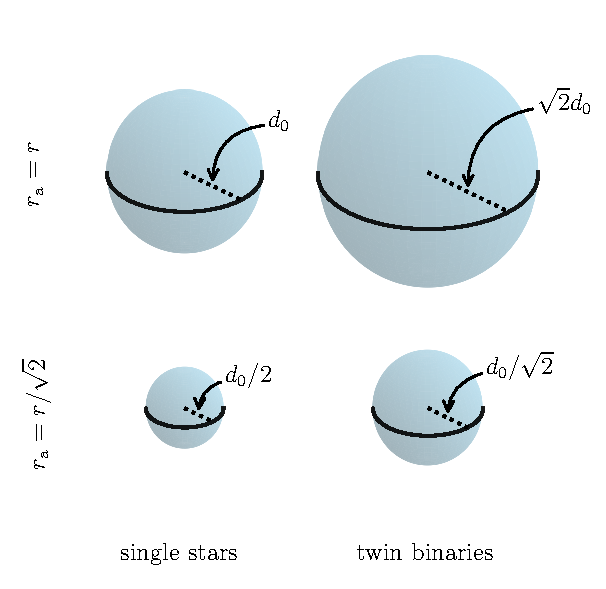
\includegraphics[width=0.6\textwidth]{figures/visualize_volumes.pdf}
    \end{center}
    \caption{
        Searchable volumes for single stars ({\it left}) and twin
        binaries ({\it right}), assuming that all stars have the same
        mass, radius, and luminosity, and that all planets have the
        same radius $r\p$.
        {\it Top:} At an apparent radius $r\a=r\p$, the
        binarity-ignoring observers search twin binaries out to a
        distance $\sqrt{2}$ times greater than they search single
        stars.  Because the transit depths are diluted, there are no 
        planets in twin binaries with $r\a=r\p$.
        {\it Bottom:} At $r\a=r\p/\sqrt{2}$, the observed transit
        depths are smaller by a factor of two, so the maximum
        searchable distances are half those at $r\a=r\p$.  The only
        detected planets with $r\a=r\p/\sqrt{2}$ orbit twin binaries.
    }
    \label{fig:model_1_volumes}
\end{figure}

Since the effects of binarity are most pronounced when the two stellar
components are similar, we begin by considering a universe in which
all stars are identical, with mass $M$, radius $R$, and luminosity
$L$.  Some fraction of them exist in twin binaries. All planets have
size $r\p$.  In this scenario, stellar radii are never misclassified
because the combined light of a binary has the same color and spectrum
as a single star.  We further assume that planets occur around single
stars and members of binaries at the same rate, $\Lambda(r\p)$.

Our naive observers detect transiting planets with two different
depths. Since 
\begin{equation}
    \delta = \left(\frac{r\p}{R}\right)^2 \frac{L}{L_{\rm tot}},
    \label{eq:delta_obs_general} 
\end{equation}
one class of transit signal, with depth $(r\p/R)^2$, occurs in single
star systems. The other class, with half the depth, occurs in twin
binary systems, leading to apparent planet radii $\sqrt{2}$ smaller
than the true radii.

To calculate the occurrence rate of each planet type, our observers
identify the ``stars'' from their survey that appear to have been
searched for signals of each depth.  These transits are detected
within a certain maximum
distance~\citep[see][]{pepper_using_2003,pepper_searching_2005}, which
from Equation~\ref{eq:S_N_thresh} scales as
\begin{equation}
  d_{\rm max} \propto \delta \, L_{\rm tot}^{1/2}.
  \label{eq:dmax}
\end{equation}
Assuming that stars are uniformly distributed in space, the number of
searchable stars $N_\star$ is proportional to
\begin{equation}
    N_\star \propto n \delta^3 L_{\rm tot}^{3/2},
\label{eq:N_searchable_prop}
\end{equation}
where $n$ is the number per unit volume of single or binary star
systems. 

When selecting sources that appear to have been searched, the
observers admit some binaries.  Since the binaries are twice as
luminous as singles, at fixed $\delta$ they are included out to a
distance that is larger by a factor of $\sqrt{2}$.  To detect the
half-strength signal, the observers need the noise level to be lower
by a factor of two, which means the flux must be four times higher
than that of a single star at distance $d_0$.  This is true of single
stars within a distance $d_0/2$, and binaries within a distance
$d_0\sqrt{2}/2$.  The searchable volumes are illustrated in
Figure~\ref{fig:model_1_volumes}.

Putting it all together, the {\it apparent} occurrence rate
$\Lambda\a$ of planets of radius $r\p$ will be
\begin{equation}
    \Lambda\a(r\p) = 
        \frac{\Lambda(r\p) \, n\s d_0^3}
        {n\s d_0^3 + n\b (d_0\sqrt{2})^3}
    \label{eq:rate_at_rp}
\end{equation}
where $n\s$ and $n\b$ are the number densities of single and binary
star systems, respectively.  This apparent rate is larger than the
true rate by a factor
\begin{equation}
    \frac{\Lambda\a(r\p)}{\Lambda(r\p)} = 
        \frac{1}{1 + 2^{3/2}(n\b/n\s)}.
    \label{eq:correction_rp}
\end{equation}
The observers will also claim to have discovered a class of planet
with radius $r\p/\sqrt{2}$ and an occurrence rate given by
\begin{equation}
    \frac{\Lambda\a(r\p/\sqrt{2})}{\Lambda(r\p)}
    =
    \frac{2n\b (d_0\sqrt{2}/2)^3}
      {n\s (d_0/2)^3 + n\b (d_0\sqrt{2}/2)^3}
    =
    \frac{2\cdot2^{3/2}(n\b/n\s)}{1 + 2^{3/2}
    (n\b/n\s)}.
    \label{eq:correction_diluted_rp}
\end{equation}

\begin{figure}[!tb]
    \begin{center}
        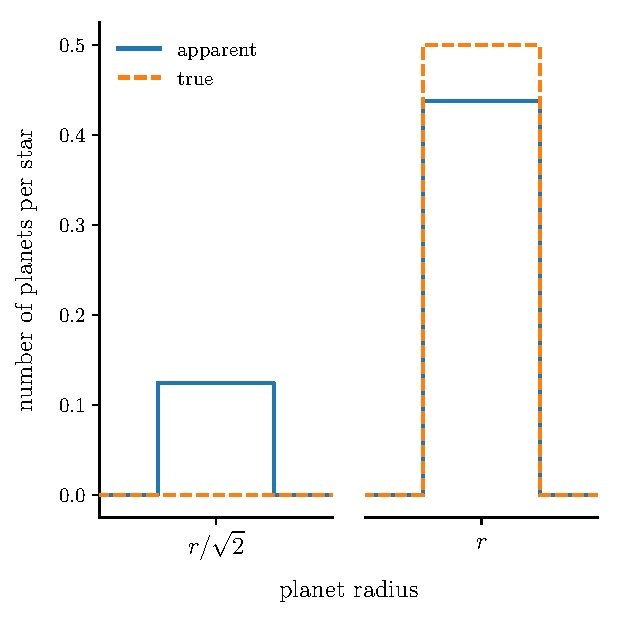
\includegraphics[width=.6\textwidth]{figures/occ_rate_vs_radius_model_1_brokenx.pdf}
    \end{center}
    \vspace{-0.5cm}
    \caption{
        Apparent occurrence rate $\Lambda\a$, and occurrence rate $\Lambda$, 
        for a model with one type of star, one
        type of planet, and twin binaries (same as
        Figure~\ref{fig:model_1_volumes}).  We assume a twin binary
        fraction of $0.05$, and that single, primary, and secondary
        stars host planets at equal rates.  If the true planet radius
        is $r\p$, all planets detected in binaries will have apparent
        radii $r\a = r\p/\sqrt{2}$; Equation~\ref{eq:ratios} gives the
        normalizations.
    }
    \label{fig:occ_rate_model_1}
\end{figure}

We can now assess the severity of these errors, given the
binary-to-single ratio $n\b/n\s$. For stars with masses from 0.7 to
1.3~$M_\odot$, \citet{raghavan_survey_2010} found the multiplicity
fraction~--~the fraction of systems in a volume-limited sample that
are multiple~--~to be 0.44.  Assuming all multiple systems are
binaries, this means
\begin{equation}
    \frac{n\b}{n\s + n\b} \approx 0.44.
\end{equation}
Of course not all of these binaries are ``twin'' binaries as we have
assumed in our simple calculation. Perhaps only a tenth of the
binaries have pairs of stars close enough in their basic properties to
produce errors as significant as those we have been considering. In
detail, this fraction depends on the binary mass ratio distribution
and stellar mass-luminosity relation (see
Section~\ref{sec:general_formula}).  Taking a leading-order estimate
of $n\b/(n\s+n\b)\approx0.05$, we find
\begin{equation}
    \frac{\Lambda\a(r\p)}{\Lambda(r\p)} = 0.87,~~
    \frac{\Lambda\a(r\p/\sqrt{2})}{\Lambda(r\p)} = 0.26.
    \label{eq:ratios}
\end{equation}
All together, the various effects produce biases of order 10\% in the
occurrence rates.  We will see that this level of error is
characteristic of many of our more complicated models as well.


\subsection{Formula Based on Apparent Rate Density}
\label{sec:model_1_density}

There is a different way to conceptualize the preceding results that
will be useful in the upcoming discussion. We now consider a spectrum
of planet sizes, $r$, and introduce the occurrence rate density
\begin{equation}
    \Gamma(r) \equiv \frac{{\rm d}\Lambda}{{\rm d}r},
    \label{eq:rate_density_defn}
\end{equation}
the number of planets per star per unit planet radius.  

The naive observers are in fact measuring $\Gamma\a(r\a)$, the {\it
apparent} occurrence rate density~--~the number of planets per star
per unit apparent radius $r\a$.  The ``apparent planet radius'' is the
radius inferred from the transit depth under the assumption that the
host star is single. The ``apparent stellar radius'' $R\a$ is
analogous.  The observed transit depth can be written $\delta =
(r\a/R\a)^2$, which from Equation~\ref{eq:delta_obs_general} gives
$r\a=r\p/\sqrt{2}$ for planets in twin binaries.  $\Gamma\a(r\a)$ is
the same as the {\it true} rate density of transit signals of
amplitude $\delta$.

We will now calculate the apparent rate density by evaluating the star
and planet counts for signals coming from single stars, primary stars
in binaries, and secondary stars in binaries.  Let $\mu$ be the ratio
between the number of searchable binary systems and the number of
searchable single systems at a particular transit depth. The number of
single and binary sources in the searched sample are then
\begin{equation}
  \frac{N_\star(r\a)}{1+\mu}~~{\rm and}~~\frac{\mu N_\star(r\a)}{1+\mu},
  \label{eq:N_searched}
\end{equation}
respectively.  Earlier we showed that due to Malmquist bias, $\mu =
2^{3/2}(n\b/n\s)$.

Suppose the occurrence rate densities for planets around
single stars, primaries, and secondaries are $\Gamma_0(r),
\Gamma_1(r)$, and $\Gamma_2(r)$, respectively. For a single planet
size,
\begin{equation}
    \Gamma_i(r) = \Lambda(r\p) \, \hat{\delta}(r-r\p),~~{\rm for}
    \ i\in\{0,1,2\},
    \label{eq:one_planet}
\end{equation} 
where $\hat{\delta}$ is the Dirac delta function.
The number of planets detected from singles, primaries, and
secondaries are then
\begin{align}
  n_{\rm det}^0(r\a)\mathrm{d}r\a &= 
      \frac{N_\star(r\a)}{1+\mu} p_{\rm tra}
      \Gamma_0(r\a)\mathrm{d}r\a,
  \label{eq:n0} \\
  n_{\rm det}^1(r\a)\mathrm{d}r\a &= 
      \frac{\mu N_\star(r\a)}{1+\mu} p_{\rm tra}
      \Gamma_1(\sqrt{2}r\a)\mathrm{d}(\sqrt{2}r\a),
	\label{eq:n1} \\
  n_{\rm det}^2(r\a)\mathrm{d}r\a &=
      \frac{\mu N_\star(r\a)}{1+\mu} p_{\rm tra}
      \Gamma_2(\sqrt{2}r\a)\mathrm{d}(\sqrt{2}r\a),
	\label{eq:n2}
\end{align}
where $n_{\rm det}^i$ is the number of detections per unit apparent
radius for each respective type of star.

Dividing the number of detections by the number of sources,
the apparent rate density reported when ignoring binarity is
\begin{equation}
  \Gamma\a(r\a) =
    \frac{1}{1+\mu}\,\Gamma_0(r\a) +
    \frac{\mu}{1+\mu}\,\sqrt{2}\,\Gamma_1(\sqrt{2}r\a) +
    \frac{\mu}{1+\mu}\,\sqrt{2}\,\Gamma_2(\sqrt{2}r\a).
	\label{eq:formula_twin_binary}
\end{equation}
If we insert Equation~\ref{eq:one_planet} and integrate over
apparent radius, this reproduces Equations~\ref{eq:rate_at_rp}
and~\ref{eq:correction_diluted_rp}.

\begin{comment}
  and inputting Equation~\ref{eq:one_planet}, we find
  \begin{align}
      \Gamma\a(r\a) &= \Lambda(r\p) \left[
      \frac{1}{1+\mu} \cdot
      \hat{\delta}(r\a-r\p)  +
      \frac{2\mu}{1+\mu} \cdot
      \delta\left(r\a-\frac{r\p}{\sqrt{2}} \right) \right].
      \label{eq:model_1_apparent_rate_density}
  \end{align}
  Integrating over $r\a$, this yields
  \begin{equation}
    \Lambda\a(r_{\rm p})=\frac{Z}{1+\mu},\quad
    \Lambda\a(r_{\rm p}/\sqrt{2})=\frac{2\mu Z}{1+\mu},
  \end{equation}
  which reproduce Equations~\ref{eq:correction_rp}
  and~\ref{eq:correction_diluted_rp}.
\end{comment}

\begin{comment}
    The ratio of the apparent to single star rate
    densities,
    \begin{equation}
        X_\Gamma(r) \equiv \left. \frac{\Gamma\a(r\a)}{\Gamma_0(r)}
          \right|_{r\a = r},
    \end{equation}
    can then be evaluated as a ``correction factor''.  At the true and
    diluted planet radii, $X_\Gamma(r\p)=1/(1+\mu)$ and
    $X_\Gamma(r\p/\sqrt{2})=2\mu/(1+\mu)$.  This yields a correction
    $X_\Gamma$ of 0.87~(0.76) if the binary fraction is 0.05~(0.10).
    All together the various effects produce biases of order 10\% in the
    occurrence rates.  
\end{comment}

\begin{comment}
    \subsection{One type of star, two types of planets}

    A simple extension to the previous example helps distinguish between
    the apparent and underlying planet populations.  Consider now a
    universe that is the same as in Section~\ref{sec:model_1}, except that
    half of planets have radii $r\p$, while the other half have radii
    $r\p/\sqrt{2}$.  The rate densities are
    \begin{equation}
        \Gamma_i(r) = \frac{Z_i}{2} \left[
        \hat{\delta}(r-r\p) + \delta\left(r-\frac{r\p}{\sqrt{2}}\right)
        \right], \quad {\rm for}\  i \in \{ 0,1,2 \},
    \end{equation}
    where $i=0$ corresponds to singles, $i=1$ to primaries, and $i=2$ to
    secondaries, and the $Z_i$'s are the number of planets per star of
    each type.

    Following an identical line of reasoning as in
    Section~\ref{sec:model_1}, the apparent rate density can be written
    \begin{align}
        \notag
        \Gamma\a(r\a) &=
        \frac{1}{2(1+\mu)} \left[
        Z_0 \cdot \hat{\delta}(r\a - r\p)
        +
        \left[Z_0 + \mu (Z_1 + Z_2)
        \right] \cdot \delta\left(r\a - \frac{r\p}{\sqrt{2}}\right) 
        \right. \\
        &\quad\quad\quad\quad\quad\quad\quad\quad+
        \left.
        \mu(Z_1 + Z_2) \cdot \delta\left(r\a - \frac{r\p}{2}\right)
        \right].
        \label{eq:two_radii_twins}
    \end{align}
    Just as in Equation~\ref{eq:model_1_apparent_rate_density}, the
    $N_\star^0(r\a)$ terms cancel, leaving only the $\mu$ weights.
    However, there are now three detected planet sizes.  Also different is
    that two populations contribute at $r\a = r\p/\sqrt{2}$: the first
    population is singles with $r=r\p/\sqrt{2}$, and the second is twin
    binaries with $r=r\p$.  Both populations are detected out to the same
    maximum searchable distance.  More generally, at any given apparent
    radius, there will be contributions from both singles, primaries, and
    secondaries~---~but the relative weights between these contributions
    will depend on the underlying occurrence rates.
\end{comment}

%%%%%%%%%%%%%%%%%%%%%%%%%%%%%%%%%%%%%%%%%%%%%%%%%%%%%%%%%%%%%%%%%%%%%%%%%%%%%%%
%%%%%%%%%%%%%%%%%%%%%%%%%%%%%%%%%%%%%%%%%%%%%%%%%%%%%%%%%%%%%%%%%%%%%%%%%%%%%%%
\section{General formula for apparent occurrence rate}
\label{sec:general_formula}

To generalize the procedure of Section~\ref{sec:model_1_density} for
binaries with varying light ratios, we consider an SNR-limited survey
in which stars can have arbitrary properties.  We assume that there
are some functions $L(M)$ and $R(M)$ that specify a star's luminosity
and radius in terms of its mass. We also presume that the observers
know the masses of every single and primary star, and that they assign
each binary system the properties of its primary.  Finally, we take
the volume-limited distribution of binary mass ratios, $f(q)$, to be
independent of the primary star's mass.

We want an equation for $\Gamma\a(r\a,M\a)$, the apparent rate density
at each apparent planet radius and apparent stellar mass\footnote{By
assumption, the apparent stellar mass for single star systems is the
true mass. For binary systems, the apparent mass is the mass of the
primary.}.
Similar to Equation~\ref{eq:rate_density_defn}, we define
$\Gamma(r,M)$ as the number of planets per star, per unit planet radius,
per unit stellar mass.  Due to the varying binary mass ratios, we need
the following modifications to Equation~\ref{eq:formula_twin_binary}:
%
\begin{enumerate}
%
\item The Malmquist bias is different. The ratio between the number of
binary and single systems for which a transit of depth $\delta$ is
detectable, $\mu$, has changed.  At any $(r\a,M\a)$ pair, the number
of binary systems in the searchable volume with mass ratio $(q,
q+\mathrm{d}q)$ is now
\begin{equation}
    {N_\star(r\a)\over{1+\mu}} \, {n_{\rm b}\over n_{\rm s}}
    \left[{L_{\rm tot}(M\a, q) \over L(M\a)}\right]^{3/2}
    f(q)\,\mathrm{d}q,
    \label{eq:N_binaries}
\end{equation}
where $\mu$ is given by
\begin{equation}
    \mu= 
    %\frac{N_\star^{\rm b}(r\a)}{N_s^0(r\a)}=
    \int_0^1 {n_{\rm b}\over n_{\rm s}}\left[{L_{\rm tot}(M\a, q)
    \over L(M\a)}\right]^{3/2} f(q)\,\mathrm{d}q.
    \label{eq:mu_general}
\end{equation}
Binaries with larger mass ratios are overrepresented by a factor of
$\left[{L_{\rm tot}(M\a, q)/L(M\a)}\right]^{3/2}$ because the
sample of searchable binaries is magnitude-limited.  To obtain
the number of binary systems searched at each $(r\a,M\a)$ pair,
Equation~\ref{eq:N_binaries} needs to be integrated over $q$.  It
can then replace ${\mu N_\star(r\a)/(1+\mu)}$ in
Equations~\ref{eq:n1} and~\ref{eq:n2}.

\item The apparent radius of a planet in a binary system now depends
on whether the host star is the primary or the secondary. When the host
is the primary, we write
$r=\mathcal{D}_1 r\a$, where
\begin{equation}
    \mathcal{D}_1
    = \left( \frac{ L_{\rm tot}(M\a, q)}{ L(M\a) } \right)^{1/2}.
    \label{eq:dil_1}
\end{equation}
When the host is the secondary, $r=\mathcal{D}_2 r\a$, and the
ratio between the assumed and true stellar radii must be included:
\begin{equation}
  \mathcal{D}_2
  = \frac{R(qM\a)}{R(M\a)}
    \left( \frac{L_{\rm tot}(M\a, q)}{L(qM\a)} \right)^{1/2}.
  \label{eq:dil_2}
\end{equation}

\item Since the observers assign binaries the properties of the
primary, the transit probability for planets orbiting secondaries is
over-estimated. At a fixed orbital period, this changes
$p_{\rm tra}$ in Equation~\ref{eq:n2} by a factor of
\begin{equation}
  {R(qM\a) \over R(M\a)}q^{-1/3}.
\end{equation}

\item The contribution to the apparent rate density from
secondaries now depends on the mass of the secondary, $qM\a$. The
associated measure on the right-hand side of
Equation~\ref{eq:n2} becomes ${\rm d}(qM\a)$, and gives rise to an
extra multiplicative factor of $q$.


\end{enumerate}

Taking these modifications into account, a general formula for the
apparent rate density follows:
\begin{align}
    \notag
    \Gamma\a(r\a,M\a) &= \frac{1}{1+\mu}
    \left\{ \Gamma_0(r\a, M\a)+ 
    \frac{n\b}{n\s}
    \left[ \int_0^1 \mathrm{d}q \,
           \mathcal{D}_1^3 f(q)\cdot
           \mathcal{D}_1 \Gamma_1(\mathcal{D}_1r\a, M\a)\,
    \right.   
    \right. \\
    & \quad\quad\quad\quad\quad \left.\left.
    +\int_0^1 {\rm d}q\, 
         \mathcal{D}_1^3 f(q)\cdot q \mathcal{D}_2
         \Gamma_2(\mathcal{D}_2r\a, qM\a)\cdot
         \frac{R(qM\a)}{R(M\a)} q^{-1/3}
    \right] \right\}.
    \label{eq:general_Gamma_a}
\end{align}
We give an alternative derivation in the
\hyperref[sec:appendix]{Appendix}.
With the definition of $\mu$ in Equation~\ref{eq:mu_general},
Equation~\ref{eq:general_Gamma_a} can also be expressed as
\begin{align}
    \notag
    \notag
    \Gamma\a(r\a,M\a)
    &= 
    {1\over 1+\mu}
    \left[
       \Gamma_0(r\a, M\a) \phantom{\frac{1}{1}}
       \right.&\\
       &\quad\quad \left.+\mu
       \left\langle
       \mathcal{D}_1\Gamma_1\left(\mathcal{D}_1r\a, M\a\right)
       +
       {q \mathcal{D}_2}\Gamma_2\left(\mathcal{D}_2r\a,
       qM\a\right) \cdot {R(qM\a) \over R(M\a)}q^{-1/3}
       \right\rangle
    \right],
\end{align}
where the angle brackets denote averaging over $\mathcal{D}_1^3f(q)$.
Summarized, the apparent rate density is a weighted sum of the rate
densities from singles, primaries, and secondaries.  The weights are
determined by the fraction $\mu$ and mass ratio distribution
$\mathcal{D}_1^3f(q)$ of binaries {\it in the searchable volume}.  The
fraction $\mu$ gives the relative contributions from singles and
binaries, and $\mathcal{D}_1^3 f(q)$ applies a Malmquist bias for
binaries that are brighter.  A final correction for secondaries
accounts for the overestimated transit probability.

%%%%%%%%%%%%%%%%%%%%%%%%%%%%%%%%%%%%%%%%%%%%%%%%%%%%%%%%%%%%%%%%%%%%%%%%%%%%%%%
%%%%%%%%%%%%%%%%%%%%%%%%%%%%%%%%%%%%%%%%%%%%%%%%%%%%%%%%%%%%%%%%%%%%%%%%%%%%%%%

\section{Realistic Star and Planet Distributions}
\label{sec:more_complicated}

We will now apply our general equation for the apparent rate density
(Equation~\ref{eq:general_Gamma_a}) to study the impact of
unrecognized binaries in regimes of observational interest.  In the
following, we write the rate density for each type of star,
$\Gamma_i(r)$, as the product of a shape function, normalized to
unity, and a constant:
\begin{equation}
    \Gamma_i(r) = Z_i f_i(r), \quad {\rm for\ }i\in\{0,1,2\},
\end{equation}
where the respective indices correspond to single stars, primaries of
binaries, and secondaries of binaries.  The normalizations $Z_i$ are
each system type's occurrence rate $\Lambda_i$, integrated over all
planetary radii. In other words, they are number of planets per
single, primary, or secondary star.  Our main interest is in
varying the radius shape function and the relative values of the
integrated occurrence rates. We will also briefly mention shape
functions in stellar mass.  For analytic simplicity, we will assume
throughout this section that stars are a one-parameter family, given
by $L \propto M^\alpha \propto R^\alpha$.  Applying these power laws
to Equations~\ref{eq:dil_1} and~\ref{eq:dil_2}, we find
\begin{equation}
  \mathcal{D}_1
  =  (1+q^\alpha)^{1/2}~~{\rm and}~~\mathcal{D}_2
  = q(1+q^{-\alpha})^{1/2}
\end{equation}
for the radius dilution prefactors.

%%%%%%%%%%%%%%%%%%%%%%%%%%%%%%%%%%%%%%%%%%%%%%%%%%%%%%%%%%%%%%%%%%%%%%%%%%%%%%%
\subsection{Power law planet radius distribution}
\label{sec:model_2}

\subsubsection{Twin binaries}
As a first step, we return to the case where all binaries are twins.
However, we now let the planet radius distribution be a power law,
\begin{equation}
    \Gamma_i(r) = Z_i f(r) = Z_i r^\gamma/\mathcal{N}_r,
\end{equation}
for $\mathcal{N}_r$ the shape function's normalization.  Applying
Equation~\ref{eq:general_Gamma_a} gives the resulting apparent rate
density,
\begin{equation}
    \Gamma\a(r\a) = \frac{r\a^{\gamma}}{\mathcal{N}_r} \left[
    \frac{Z_0}{1+\mu}
    +
    2^{\frac{\gamma+1}{2} } \frac{\mu}{1+\mu} \left(Z_1 + Z_2
    \right)
    \right].
    \label{eq:model5_apparent_rate_density}
\end{equation}
Under these assumptions, twin binaries simply shift the apparent
radius distribution: $\Gamma\a(r\a) \propto r\a^\gamma$.  As in
Section~\ref{sec:model_1}, $\mu = 2^{3/2} n\b/n\s$.  If planet
occurrence is independent of system multiplicity, the ``correction
factor'' relative to the rate density for singles is
\begin{align}
    \frac{\left. \Gamma\a(r\a)\right|_{r\a= r}}{\Gamma_0(r)} 
    &=
    \frac{1 + 2^{\frac{\gamma+3}{2}}\mu}{1 + \mu}.
    \label{eq:power_law_correction}
\end{align}
For a binary fraction of $0.1$, $\mu\approx 0.15$. Taking
$\gamma=-2.92$ from \citet{howard_planet_2012},  we find that the
apparent rate density is a mere 0.4\% larger than the rate density of
single stars.  Fortuitously, the exponent of the radius distribution
is close to $-3$, and the errors from neglecting binaries almost
entirely cancel out.

The above estimate cannot apply at small radii, since the shape
function diverges. \citet{howard_planet_2012}'s results indicate that
a single power law fits the planet radius distribution for radii
greater than $2r_\oplus$.  Similarly, there should be an upper radius
limit, $r_{\rm u}$, to the radius distribution, perhaps around
$24r_\oplus$ based on the most inflated hot Jupiters.  Imposing an
upper cut-off of $r_{\rm u}$ would lead to smaller values of the
apparent rate density down to $r_{\rm u}/\sqrt{2}$, compared to a
power law without the cut-off.  We are not particularly interested in
this effect because hot Jupiter occurrence rates are poorly described
by a power law (see Section~\ref{sec:further_models}).  All told, if
our assumptions are applicable to real transit surveys,
Equation~\ref{eq:power_law_correction} suggests that for apparent
radii from $2r_\oplus$~to~$17r_\oplus$, unrecognized binaries are a
minor source of systematic error.


%%%%%%%%%%%%%%%%%%%%%%%%%%%%%%%%%%%%%%%%%%%%%%%%%%%%%%%%%%%%%%%%%%%%%%%%%%%%%%%
\subsubsection{Binaries with power law mass ratio distribution}
\label{sub:powerlaw_varying_binaries}

\begin{figure}[!tb]
    \centering
    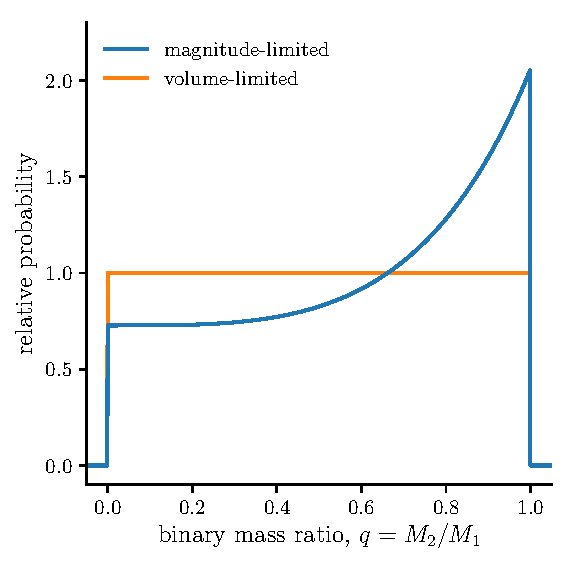
\includegraphics[width=0.6\textwidth]{figures/mass_ratio_distribution.pdf}
    \caption{
        The mass ratio distribution for a magnitude-limited sample of
        binary stars, in which the underlying volume-limited
        distribution is uniform, qualitatively similar to Figure~16 of
        \citet{raghavan_survey_2010}.  At a given observed transit
        depth, the searchable binaries in a transit survey are
        magnitude-limited. For this figure, we assume $L\propto
        M^{3.5}$.
    }
    \label{fig:q_distribn_mag_limited}
\end{figure}

To check whether non-twin binaries change the preceding result, we now
consider a distribution of binary mass ratios.  Specifically, we take
$f(q) = q^\beta/\mathcal{N}_q$, for $\mathcal{N}_q$ the normalization.
This changes $\mu$ from the twin binary case;
Equation~\ref{eq:mu_general} simplifies to
\begin{equation}
    \mu = \frac{n\b}{n\s} \frac{1}{1+\beta}
    \int_0^1 (1+q^\alpha)^{3/2}q^\beta\,{\rm d}q.
    \label{eq:mu_power_law_q}
\end{equation}
For the $\beta=0$ case, this equation means there will be more
twin-like binaries than faint binaries in the sample of stars
that are searched at any transit depth
(Figure~\ref{fig:q_distribn_mag_limited}). 

The rate density now varies not only with planet radius, but also
host star mass.  We can absorb this dependence into a power law,
\begin{equation}
    \Gamma_i(r,M) = Z_i \, \frac{r^\gamma}{\mathcal{N}_r} \,
    \frac{M^\zeta}{\mathcal{N}_M},
\end{equation}
where $Z_i$ is dimensionless, and the normalization constants carry
the units.% (each side has units $[r^{-1} M^{-1}]$).

Our main interest is in the apparent rate density's radius
dependence.  Marginalizing Equation~\ref{eq:general_Gamma_a} over
apparent stellar mass, we find that when all stars host the same number
of planets,
\begin{align}
    %see annoying_q_factor_dec22.pdf for derivation
    \notag
    \frac{\left.\Gamma\a(r\a)\right|_{r\a= r}}{\Gamma_0(r)} 
    &=
    \frac{1}{1+\mu}
    \left[
      1 + \frac{1}{\mathcal{N}_q} \frac{n\b}{n\s}
    \left(
      \int_0^1 {\rm d}q\,q^\beta (1+q^\alpha)^{\frac{\gamma+4}{2}} +
      \right.
      \right. \\
      %isn't latex great?
      &\quad\quad\quad\quad\quad\quad\quad\quad\quad\quad\quad
      \left.\left.
      \int_0^1 {\rm d}q\,q^{\beta+\gamma+\frac{5}{3}} 
      (1+q^\alpha)^{\frac{3}{2}}
      (1+q^{-\alpha})^{\frac{\gamma+1}{2}}
    \right)
    \right],
    \label{eq:powerlaw_vary_binary}
\end{align}
where $\zeta$ does not appear because of the marginalization over
$M\a$.  For $\alpha = 3.5$, $\beta=0$, $\gamma=-2.92$, the
summed integrals in Equation~\ref{eq:powerlaw_vary_binary} give
$(\ldots)\approx 1.503$. %171211_model_integrals.nb
For $n\b / (n\b + n\s)=0.44$, this yields $\Gamma\a/\Gamma_0 = 1.048$.
The apparent rate density is 4.8\% larger than the rate density around
singles.  Considering only twin binaries gave us good intuition: for
apparent radii from $2r_\oplus$ to $17r_\oplus$, binarity influences
apparent planet occurrence rates around Sun-like stars at the level of
a few percent.



%%%%%%%%%%%%%%%%%%%%%%%%%%%%%%%%%%%%%%%%%%%%%%%%%%%%%%%%%%%%%%%%%%%%%%%%%%%%%%%
\subsection{Varying stars; broken power law planet radius distribution}
\label{sec:model_3}

\begin{figure}[!t]
    \centering
    \epsscale{1.15}
    \plottwo{figures/int_rate_density_vs_radius_model_3_rpu_22.5_manyZs.pdf}{figures/int_occ_rate_vs_radius_model_3_rpu_22.5_manyZs.pdf}
    \caption{
        {\it Left:} apparent rate density ($\Gamma\a$) and rate density for 
        single stars ($\Gamma_0$). {\it Right:} apparent occurrence
        rate ($\Lambda\a$) and single star occurrence rate
        ($\Lambda_0$), over $0.5r_\oplus$ bins.  The true planet
        radius distribution is specified by
        Equation~\ref{eq:model3_radius_distribution}.  This model
        assumes that the observer knows the true properties of all the
        singles and primaries, and that the volume-limited mass ratios
        of secondaries are drawn from a uniform distribution. Further,
        we take $Z_0=Z_1=0.5$ throughout; $Z_0,Z_1,Z_2$ are the number
        of planets per single, primary, and secondary star.  The rate
        and rate density are related by $\Lambda|_a^b =
        \int_{a}^{b}\Gamma\,{\rm d}r$.
    }
    \label{fig:occ_rate_model_3_log}
\end{figure}

Though the details of the planet radius distribution $\Gamma_i(r)$ at
$r<2r_\oplus$ are currently an active topic of research, by making
plausible assumptions we can investigate how neglecting binarity might
bias measurements in this regime.  For instance, consider a broken
power-law:
\begin{align}
    f(r)
    &\propto
    \left.
    \begin{cases}
        r^\gamma & \text{for } r\geq 2r_\oplus \\
        {\rm constant} & \text{for } r\leq2r_\oplus.
    \end{cases}
    \right.
    \label{eq:model3_radius_distribution}
\end{align}
At apparent radii $r\a > 2r_\oplus$, the apparent rate density in
this model is the same as that in
Section~\ref{sub:powerlaw_varying_binaries}.  At smaller apparaent
radii the equations are tedious, but still tractable.
For simplicity, we insert Equation~\ref{eq:model3_radius_distribution}
into Equation~\ref{eq:general_Gamma_a}, and integrate using a computer
program. We refer the interested reader to our online
implementation\footnote{\url{https://github.com/lgbouma/binary_biases}}.
The output, shown in Figure~\ref{fig:occ_rate_model_3_log}, is
validated using analytic predictions in the $r\a > 2r_\oplus$ and the
$r\a < 2r_\oplus/\sqrt{2}$ regimes.  As before, $L\propto M^\alpha
\propto R^\alpha$, and $\alpha=3.5$, $\beta=0$, $\gamma=-2.92$.  

\paragraph{The rate of Earth analogs} The immediately arresting result
is a ``bump'' in the apparent rate density at apparent radii below
$2r_\oplus$: the true rate for singles is less than the apparent rate.
If secondaries host as many planets as single stars, the occurrence of
these small planets is overestimated by about $50\%$.  The magnitude
of the systematic error decreases if there are fewer planets around
secondaries; if secondaries host no planets at all, the apparent rate
is overestimated by only $10\%$.  

\paragraph{Hot Jupiter occurrence rates}
By integrating the rate density from
Figure~\ref{fig:occ_rate_model_3_log}, we can compare the apparent hot
Jupiter occurrence rate with the true rate for singles.  The
difference between the rates is largest when secondaries host no
planets. In that case, we find $\Lambda_{{\rm HJ},0}/\Lambda_{\rm
HJ,a} = 1.13$, where
\begin{equation}
    \Lambda_{\rm HJ,a} =
      \int_{8r_\oplus}^{\infty} \Gamma\a(r\a)\,{\rm d}r\a,~~{\rm
      and}~~
    \Lambda_{\rm HJ,0} =
      \int_{8r_\oplus}^{\infty} \Gamma_0(r)\,{\rm d}r.
\end{equation}
%occ_rate_vs_radius_model_3_withtext_Zsub2_0.00_rpu_22.5.pdf
If secondaries host half as many planets as single stars, then
$\Lambda_{{\rm HJ},0}/\Lambda_{\rm HJ,a} = 1.06$.  We pay further
attention to the issue of hot Jupiter occurrence rates in
Section~\ref{sec:further_models}.

\paragraph{Fraction of detected planets from a given source}

\begin{figure}[!t]
    \centering
    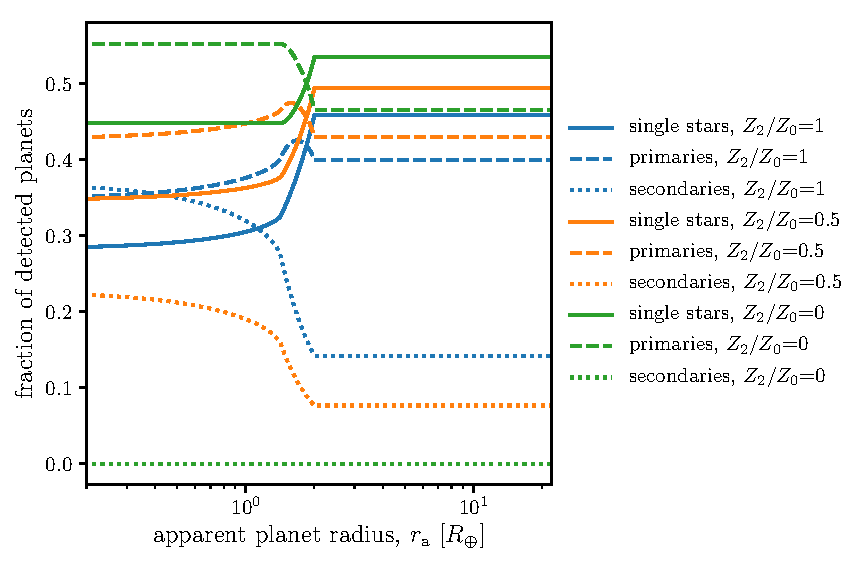
\includegraphics[width=\textwidth]{figures/ndet_vs_radius_logx_model_3_fraclines_rpu_22.5_manyZs.pdf}
    \caption{
        Fraction of detected planets at a given apparent planet radius
        that orbit single stars (solid lines), primaries of binaries
        (dashed lines), and secondaries of binaries (dotted lines).
        We assume that single stars and primaries have the same number
        of planets per star, and that the true planet radius
        distribution is a broken power law
        (same as Figure~\ref{fig:occ_rate_model_3_log}).
    }
    \label{fig:frac_model_3}
\end{figure}

A common situation during transit survey follow-up is for
high-resolution imaging to reveal multiple stars in a system that
shows planetary transits.  It is often impossible to rule which star
hosts the detected planet.  One would intuitively expect that the
primary star would be the more likely host because at fixed planet
size, planetary transits around secondaries have smaller amplitudes
(Equations~\ref{eq:dil_1} and~\ref{eq:dil_2} imply
$\mathcal{D}_2>\mathcal{D}_1$, if $\alpha=3.5$).  However, this
reasoning is qualitative, and its assumptions might not always hold.

Our formalism lets us calculate the relative probability that a
detected planet orbits a single, primary, or secondary star in a more
general manner.  To perform the calculation, we use expressions given
in the appendix for the number of detections coming from each type of
system (Equations~\ref{eq:n_det_0},~\ref{eq:n_det_1},
and~\ref{eq:n_det_2}).  We then divide out by the total number of
detections at each apparent radius.  Figure~\ref{fig:frac_model_3}
shows the result: if high-resolution imaging reveals a source with
transits to be a binary system, the detected planet does usually orbit
the primary.

If the apparent radius of the system is above $2r_\oplus$, and planets
exist about primaries and secondaries at equal rates, then the planet
is $3$ times more likely to orbit the primary than the
secondary.  If secondaries host half as many planets as primaries,
then a detected planet is $5$ times more likely to orbit the
primary.

The situation for apparent radii below $2r_\oplus$ is more nuanced.
For the two cases in which secondaries host fewer planets than
primaries, detected planets in binaries are still always more likely
to orbit the primary.  However, if planets exist at the same rate in
primaries and secondaries, then below apparent radii of $0.4r_\oplus$,
more of the detected planets in binaries come from secondaries~--~they
have all been diluted down from larger true planetary radii.
Rephrased, going from apparent radii of $2r_\oplus$~to~$1.4r_\oplus$,
the fraction of detected planets with binary companions increases by
anywhere from $6\%$~to~$12\%$, depending on the relative occurrence of
planets about primaries and secondaries.  We compare this prediction
with recent observations in Section~\ref{sec:discussion}.
%~\footnote{
%The increase can be derived analytically.  Let the fraction of total
%detected planets from primaries at a given apparent radius be
%$F_1(r\a)$, so $F_1(r\a) \equiv n_{\rm det}^1(r\a)/n_{\rm det}^{\rm
%tot}$.  Let the analogous quantity for secondaries be $F_2(r\a)$.  In
%the planet-less secondaries case ($F_2(r\a)=0$), one can analyze
%Eqs~\ref{eq:n_det_0} and~\ref{eq:n_det_1} semi-analytically and show
%that $F_1(2r_\oplus/\sqrt{2})/F_1(2r_\oplus) \approx 1.19$.
%check_companion_fractions.py, and LB's notes 2017/12/21.0 }.



%%%%%%%%%%%%%%%%%%%%%%%%%%%%%%%%%%%%%%%%%%%%%%%%%%%%%%%%%%%%%%%%%%%%%%%%%%%%%%%
\subsection{Further models: radius gaps, Gaussian HJ distributions}
\label{sec:further_models}

The radius distribution specified by
Equation~\ref{eq:model3_radius_distribution} misses some important
features revealed by state of the art planet occurrence studies.

\paragraph{Precise features of the radius valley}

\begin{figure}[!t]
    \centering
    \epsscale{1.15}
    \plottwo{figures/int_rate_density_vs_radius_model_4_xcut_manyZs.pdf}{figures/int_occ_rate_vs_radius_model_4_xcut_manyZs.pdf}
    \caption{
        {\it Left:} rate density and {\it right:} rate as a function
        of planet radius in a model with a radius gap
        (Equation~\ref{eq:model4_radius_distribution}).  Other than
        the intrinsic radius distribution, this model has the same
        assumptions as Figure~\protect\ref{fig:occ_rate_model_3_log}.
    }
    \label{fig:model_4}
\end{figure}

\citet{fulton_california-_2017} recently reported a ``gap'' in the
radius-period
plane~\citep{petigura_california-kepler_2017,johnson_california-kepler_2017}.
The existence of the gap has been independently corroborated from a
sample of KOIs with asteroseismically-determined stellar
parameters~\citep{van_eylen_asteroseismic_2017}.  Precise measurement
of the gap's features, in particular its width, depth, and shape, will
require accurate occurrence rates.  To illustrate binarity's role in
this problem, we make identical assumptions as in
Section~\ref{sec:model_3}, but instead assume an intrinsic radius
distribution
\begin{align}
    f(r)
    &\propto
    \left.
    \begin{cases}
        r^\gamma & \text{for } r\geq 2r_\oplus, \\
        0 & \text{for } 1.5r_\oplus < r < 2r_\oplus, \\
        {\rm constant} & \text{for } r\leq1.5r_\oplus.
    \end{cases}
    \right.
    \label{eq:model4_radius_distribution}
\end{align}
Figure~\ref{fig:model_4} shows the resulting true and apparent rates.
If left uncorrected, binarity makes the gap appear more shallow, and
flattens the step-function edges.  Of course, effects unrelated to
binarity would also ``blur'' the gap in the planet radius dimension.
In particular, the valley's period-dependence is almost certainly not
flat \citep{van_eylen_asteroseismic_2017,owen_evaporation_2017}.  This
means that any study measuring the gap's width or depth while
accounting for binarity must either perform tests at fixed orbital
period, or else marginalize over period and account for the associated
blurring in the planet radius dimension.


\paragraph{The HJ distribution is not a power law}

In the recent study by~\citet{petigura_CKS_2017}, hot Jupiters appear
as an island in period-radius space, rather than as a continuous
component of a power law distribution.  This means that the apparent
HJ rates computed in Section~\ref{sec:model_3} are probably
inaccurate.  Instead, let us consider a Gaussian radius shape
function,
\begin{equation}
    f(r) \propto \exp \left( -\frac{(r-\bar{r})^2}{2\sigma^2} \right),
\end{equation}
with $\bar{r} = 14r_\oplus$ and $\sigma = 2r_\oplus$.  As always,
$\Gamma_i(r) = Z_i f(r)$.  We then compute $\Gamma\a(r\a)$, and plot
it in Figure~\ref{fig:gaussian_HJ}.  Integrating over $r\a >
8r_\oplus$ to find hot Jupiter rates, we find the opposite effect as
in the power law model.  If secondaries host any planets at all, the
apparent HJ rate is {\it greater} than the true rate for singles.  For
instance, if the hot Jupiter rate about secondaries and singles
is equal, then $\Lambda_{{\rm HJ},0}/\Lambda_{\rm HJ,a} = 0.81$.
%int_rate_density_vs_radius_model_7_withtext*manyZs.pdf
Qualitatively, the apparent HJ rate is greater than the true rate for
singles because binary systems have extra uncounted stars that
yield hot Jupiter detections.


\begin{figure}[!tb]
    \centering
    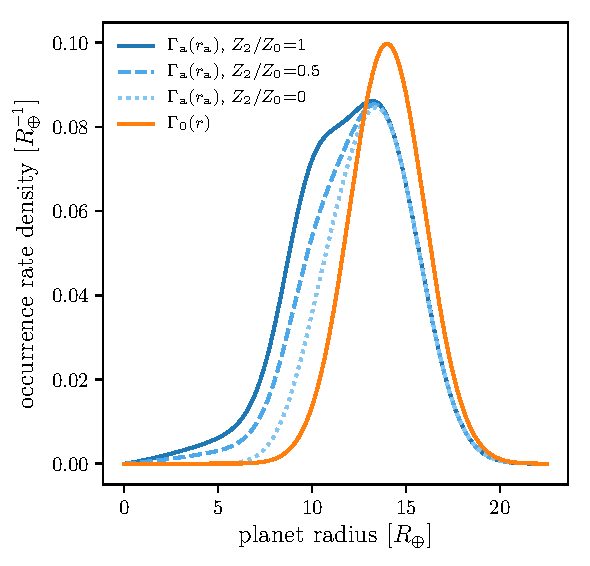
\includegraphics[width=.6\textwidth]{figures/int_rate_density_vs_radius_model_7_rpu_22.5_manyZs.pdf}
    \caption{
        Rate density for a population of planets with true radii $r$
        drawn from a Gaussian with mean $14r_\oplus$ and standard
        deviation $2r_\oplus$.  This is similar to the hot Jupiter
        distribution presented by~\citet{petigura_CKS_2017}.
    }
    \label{fig:gaussian_HJ}
\end{figure}


%%%%%%%%%%%%%%%%%%%%%%%%%%%%%%%%%%%%%%%%%%%%%%%%%%%%%%%%%%%%%%%%%%%%%%%%%%%%%%%
%%%%%%%%%%%%%%%%%%%%%%%%%%%%%%%%%%%%%%%%%%%%%%%%%%%%%%%%%%%%%%%%%%%%%%%%%%%%%%%

\section{Discussion}
\label{sec:discussion}


\paragraph{How bad is ignoring binarity?}
This study has shown that under a reasonable set of simplifying
assumptions, ignoring binarity introduces systematic errors to star
and planet counts in transit surveys, which then biases derived
occurrence rates.  Thus far, occurrence rate calculations\footnote{ A
list of occurrence rate papers is maintained at
\url{https://exoplanetarchive.ipac.caltech.edu/docs/occurrence_rate_papers.html}
} using transit survey data have mostly ignored stellar
multiplicity~\citep[\textit{e.g.},][]{howard_planet_2012,fressin_false_2013,foreman-mackey_exoplanet_2014,dressing_occurrence_2015,burke_terrestrial_2015}.
For {\it Kepler} occurrence rates specifically, it seems that no one
has yet carefully assessed binarity's importance, or lack thereof.
This study does not resolve the problem; it only suggests the
approximate scale of the systematic errors.  Section~\ref{sec:model_2}
suggests that for apparent radii above $2r_\oplus$, binarity can be
ignored down to a precision of a few percent.  For apparent radii
below $2r_\oplus$, the picture is less forgiving:
Section~\ref{sec:model_3} suggests that the apparent rates around
single stars could be overestimated by as much as 50\%.

\paragraph{The rate of Earth analogs}
\citet{youdin_exoplanet_2011},~\citet{petigura_prevalence_2013},~\citet{dong_fast_2013},~\citet{foreman-mackey_exoplanet_2014},
and~\citet{burke_terrestrial_2015} have found that between $0.03$ and
$1$ Earth-like planets exist per Sun-like star, depending on
assumptions that are made when calculating the
rate~\citep[see][Figure~17]{burke_terrestrial_2015}.  Assuming a
broken power-law, we showed that unrecognized binaries could cause
overestimates in the rate of Earth analogs of up to 50\%.  This
systematic effect is smaller than the other factors that currently
dominate the dispersion in $\eta_\oplus$ measurements.  If future
analyses determine absolute values of $\eta_\oplus$ to better than a
factor of two, binarity will likely merit closer attention.

One caveat is that none of our models included the rate density's
period-dependence. However, binaries with separations $\lesssim
10\,{\rm AU}$ could provoke dynamical instabilities, leading to fewer
Earth-like planets per
star~\citep[\textit{e.g.},][]{holman_long-term_1999,wang_influence_2014,
kraus_impact_2016}.  This would affect transit survey measurements of
$\eta_\oplus$ beyond our rough estimate.

\paragraph{Hot Jupiter rate discrepancy}
While unresolved binaries may bias $\eta_\oplus$ measurements, our
approach suggests that they do not influence the hot Jupiter rate
discrepancy.  The ``discrepancy'' is that RV surveys find roughly
twice as many hot Jupiters per Sun-like star as do transit surveys
(roughly $1\%$~vs.~$0.5\%$, respectively).  We summarize hot
Jupiter rates reported by different surveys in
Table~\ref{tab:hj_rates}.

Though the disagreement is only weakly significant ($<3\sigma$), one
reason to expect a difference is that the RV sample is biased towards
metal-rich stars, which host more giant
planets~\citep{santos_spectroscopic_2004,fischer_planet-metallicity_2005,gould_frequency_2006}.
Investigating the discrepancy from the metallicty
angle,~\citet{guo_metallicity_2017} measured the {\it Kepler} field's
mean metallicity to be $[{\rm M/H}]_{\rm Kepler}= -0.045\pm0.009$,
which is lower than the California Planet Search's mean of $[{\rm
M/H}]_{\rm CPS}= -0.005\pm0.006$.  The former value agrees with that
found by \citet{dong_metallicities_2014}.  Refitting for the
metallicity exponent in $\Lambda_{\rm HJ} \propto 10^{\beta [{\rm
M/H}] }$, \citeauthor{guo_metallicity_2017}\! found $\beta = 2.1\pm
0.7$, and noted that the metallicity difference could account for
0.2\% of the needed 0.5\% difference between the measured CKS
and {\it Kepler}\ rates\footnote{ \citet{petigura_CKS_2017} recently
found $\beta = 3.4^{0.9}_{-0.8}$.  If true, this implies that
metallicity could account for about half of the hot Jupiter rate
discrepancy.  }.  \citeauthor{guo_metallicity_2017}\!  concluded
that ``other factors, such as binary contamination and imperfect
stellar properties'' must also be at play.

Radial velocity surveys usually reject visual and spectroscopic
binaries~\citep{wright_frequency_2012}, so their hot Jupiter rates are
closer to the rate for single stars than the rates reported by transit
surveys.  However, we found in Section~\ref{sec:further_models} that
when assuming a Gaussian radius distribution, apparent hot Jupiter
rates are {\it greater} than the true rate around singles: the effect
goes the wrong way.  There could be other systematic factors behind
the difference~--~but they are unlikely to be related to binarity.

%in spectroscopic follow-up of transiting planet candidates, the
%prevalence of astrophysical false-positives may also lead to a
%tendency against confirming transiting planets in binary systems.  A
%separate observational bias is that the RV surveys typically observe
%chromospherically ``quiet'' stars, which may bias their detection
%probability high~\citep{bastien_radial_2014}.

\begin{comment}
  If we believe the assumed power law radius distribution, we can ask
  whether this ``correction factor'' might help resolve the
  discrepancy.  Explicitly, we ask: what is the probability of
  \citet{wright_frequency_2012}'s result, given a rate drawn from the
  stated bounds of~\citet{petigura_CKS_2017}?  In other words, we
  first take the true HJ rate per thousand stars as $\Lambda_{\rm HJ}
  = 5.7 \pm 1.3$, with Gaussian uncertainties.  We then draw from a
  Poisson distribution and compute the probability of detecting at
  least 10 hot Jupiters in a sample of 836 stars.  Without accounting
  for binarity or metallicity, only 4\% of RV surveys would detect at
  least 10 hot Jupiters.  If we multiply $\Lambda_{\rm HJ}$ by $1.2$
  to account for~\citet{guo_metallicity_2017}'s measured metallicity
  difference between the {\it Kepler}\ field and the local solar
  neighborhood, 9\% of RV surveys would detect at least 10 hot
  Jupiters.  If we multiply once more by $1.13$ to account for
  binarity's supposed bias, we find that 14\% of RV surveys would
  detect at least 10 hot Jupiters, still suggesting a weak
  discrepancy.  This suggestion should be taken with caution, because
  it (incorrectly) assumes a power law radius distribution.
\end{comment}


\paragraph{Does a detected planet orbit the primary or secondary?}

A separate reason to address stellar multiplicity in transit surveys
is that it can radically alter the interpretation of planet candidates
on a system-by-system level.  To identify and correct for unseen
stellar companions, high-resolution imaging campaigns have surveyed
almost all {\it Kepler}\ Objects of Interest~\citep{
  howell_speckle_2011,adams_adaptive_2012,adams_adaptive_2013,horch_observations_2012,
  horch_most_2014,lillo-box_multiplicity_2012,lillo-box_high-resolution_2014,dressing_adaptive_2014,
  law_robotic_2014,cartier_revision_2015,everett_high-resolution_2015,gilliland_hubble_2015,
  wang_influence_2015,wang_influence_2015-1,baranec_robo-ao_2016,ziegler_robo-ao_2017}.
The results of these programs have been summarized
by~\citet{furlan_kepler_2017}, and they represent an important advance
in understanding the KOI sample's multiplicity statistics.

An immediate application is to reassess the radii of detected planets.
Doing so, \citet{hirsch_assessing_2017} recently found that for their
sample of KOIs in binaries, the planet radii are underestimated by
factors $r/r\a = 1.17$ if all planets orbit primaries, and $r/r\a =
1.65$ if detected planets are equally likely to orbit primaries and
singles.  This approach makes minimal assumptions about the likelihood
that a planet orbits the primary vs.~the secondary
(though~\citealt{hirsch_assessing_2017} do also consider weighting
radius corrections by planet occurrence).

Our approach provides a suggestion of how to assess the probability
that a detected planet in a binary system orbits either component.
The problem requires assuming both the underlying radius distribution,
and the relative number of planets per primary and secondary star.  We
found that for a broken power law radius distribution, with equal
occurrence rates about primaries and secondaries, detected planets in
binary systems are usually more likely to orbit the primary
(Figure~\ref{fig:frac_model_3}).  For apparent radii greater than
$2r_\oplus$, the odds of primary:secondary are 8:3.  The odds increase
for the planet to orbit the secondary increase at smaller apparent
radii, and reach 1:1 at $r\a=0.4r_\oplus$.  For {\it Kepler}, this
suggests that for almost all confirmed KOIs in multiple star systems,
the planet most likely orbits the primary.


\paragraph{Fraction of detected planets with binary companions}
A related effect is that some detected planets are more likely to be
in binary systems than others.  Notably, Figure~\ref{fig:frac_model_3}
predicts that the fraction of detected planets with binary companions
should increase by $6$~to~$12\%$ going from $2r_\oplus$ to
$1.4r_\oplus$.

In \citet{ziegler_robo-ao_2017}'s recent summary of the Robo-AO KOI
survey, they reported the fraction of planet-hosting stars with
Robo-AO detected companion stars, binned over apparent planet radii.
The fraction of KOIs with nearby stars and their $1\sigma$
uncertainties are:
\begin{itemize}
    \item Earths ($r\a < 1.6r_\oplus$): $16.3 \pm 1.0\%$, from 1480
    systems.
    \item Neptunes ($1.6r_\oplus < r\a < 3.9 r_\oplus$): $13.0 \pm
    0.8\%$, from 2058 systems.
    \item Saturns ($3.9r_\oplus < r\a < 9 r_\oplus$): $13.6 \pm 2.0\%$, from 338 systems. 
    \item Jupiters ($r\a > 9r_\oplus$): $19.0 \pm 2.8\%$, from 247 systems. 
\end{itemize} 
The uncertainties were calculated
following~\citet{burgasser_binarity_2003}.  The absolute values of the
companion fractions are lower than in the solar neighborhood at
least in part because of Robo-AO's sensitivity
(\citealt{ziegler_robo-ao_2017}'s
Figure~2;~\citealt{raghavan_survey_2010}).
%Another reason for the lower measured companion fraction could be
%that planetary systems are more rare in binary systems,
%as~\citealt{kraus_impact_2016} found for close binary companions).
The uptick in the companion rate for Jupiters is likely tied to a
large astrophysical false positive rate~\citep{santerne_sophie_2012}.
Going from Neptunes to Earths, the data suggest a weak increase in the
detected planet companion fraction, perhaps of a few percent.  It will
be interesting to see whether this effect is borne out by further
observations.


\paragraph{Connection between high-resolution imaging and occurrence rates}

Occurrence rate calculations are beginning to incorporate the results
of high-resolution imaging surveys.  For example, recent studies have
reduced contamination in the numerator of the occurrence rate by
using~\citet{furlan_kepler_2017}'s catalog to test the effects of
removing KOI hosts with known companions
(\citealt{fulton_california-_2017}; \citealt{petigura_CKS_2017}).
This is a good first step, but the denominator remains uncorrected.  

Even if the multiplicity of every star that {\it Kepler} surveyed were
known, the problem would not be solved. In this scenario, it would be
possible to tabulate planet occurrence for single and binary star
systems separately.  The number of planets per single star would
be known.  However the number of planets per primary and secondary
would still be convolved.  An observational approach to separating the
two populations might be to analyze the centroids, or the transit
durations (and thus host star densities) for a representative sample
of planets in binary systems. 

A theory-driven solution might entail probabilistic population
inference, with a parametrized model for planet populations around
primary and secondary stars.  Such an approach might be expected to
find that the primary and secondary populations are different, since
single M dwarfs host more small planets than FGK
dwarfs~\citep{dressing_occurrence_2015}.  Given the difficulty of
writing a likelihood function in a survey with systematic
biases, one possible approach might be to forward-model the survey in
the framework of approximate Bayesian
computation~\citep[\textit{e.g.},][]{morehead_understanding_2016}.


\begin{comment}
%LB: the below paragraph seems like it is just making caveats for no
%good reason. We've been explicit throughout that we have a
%restrictive set of assumptions...

  \paragraph{Practical effects: smooth detection efficiencies and finite SNR floors}
  To apply this study to real transit surveys, a few practical concerns
  become pressing.  One issue is that space-based missions with
  telemetric requirements often must select target stars.  Even if the
  selection process aims to create an SNR-limited survey,
  as~\citet{batalha_selection_2010} did for {\it Kepler}, uncertainties
  in stellar parameters and the modeled instrument performance can lead
  to deviations away from an SNR-limited stellar sample.

  Another concern is that in real transit surveys the detection
  efficiency is not a step function in SNR.  Transit survey pipeline
  detection efficiencies are usually smooth
  functions~\citep{christiansen_measuring_2016,fulton_california-_2017}.
  If we were to assume a smooth detection probability in SNR, we would
  need to appropriately weight our occurrence calculation for planets
  with low probabilities of being detected.

  The simplest way to avoid the conceptual complications of accounting
  for finite detection efficiency is to raise the SNR floor, to {\it
  e.g.,} ${\rm SNR} \approx 12$ for {\it Kepler}
  (\citealt{fulton_california-_2017}, Figure~5).  To a good
  approximation, this allows use of the boolean distinctions
  ``searchable'' and ``not searchable'' for signals of an observed depth
  (at fixed orbital period).  By making the survey strictly SNR-limited,
  rather than ``fuzzily SNR-limited'', the effects of unrecognized
  binaries become much easier to model.  Since the minimum SNR for
  detection is set arbitrarily\footnote{For example,
  {\it Kepler}'s threshold of ${\rm SNR}=7.1$ was set for there to be no
  more than one statistical false alarm across the full {\it Kepler}
  campaign~\citep{jenkins_tests_2002}. Equally valid would have been to
  insist on no more than $10^{-3}$ false alarms per survey, raising the
  detection floor.  }, this simplification would put occurrence rate
  studies on clearer conceptual ground, and facilitate the process of
  converting the apparent radius distributions into true radius
  distributions.

  Finally, our calculations ignored the fact that a transit survey's
  finite SNR floor could censor the apparent rate density. This would
  make planets with smaller apparent radii harder to detect.  Other than
  moving the small radii regime out of reach for that particular survey,
  this would not change any of our findings.

\end{comment}


\begin{comment}
%LB: the following are paragraphs from earlier discussion iterations

  To count the number of stars that
  were searched, further effort to understand the multiplicity
  statistics of KOI vs.~non-KOI stars is necessary. In particular, a
  non-KOI star high-resolution imaging effort could help estimate the
  systematic errors incurred by assuming all surveyed stars are single.
  An alternate approach would be to combine {\it Gaia} parallaxes with
  measured photometric fluxes and identify binary systems as those that
  are overluminous~\citep[\textit{e.g.},][]{widmark_inferring_2018}.

  \citet{ciardi_understanding_2015} studied the effects of stellar
  multiplicity on the planet radii derived from transit surveys.  They
  modeled the problem for {\it Kepler}\ objects of interest by
  matching a population of binary and tertiary companions to KOI
  stars, under the assumption that the KIC-listed stars were the
  primaries.  They then computed planet radius correction factors
  assuming that {\it Kepler}-detected planets orbited the primary or
  companion stars with equal probability (their Section~5).  Under
  these assumptions, they found that any given planet's radius is on
  average underestimated by a multiplicative factor of $\approx\!
  1.5$.  \citet{ziegler_robo-ao_2017} recently reported a similar mean
  radius correction factor for the multiple systems observed by the
  Robo-AO KOI survey, using the same assumption that detected planets
  are as likely to orbit the primary and the secondary.

  Of course, our model's assumptions (see the list in
  Section~\ref{sec:conclusion}) might not apply to the {\it Kepler}\
  dataset.  However if they are applicable, then for the $56\%$ of
  ``\texttt{CONFIRMED}'' KOIs\footnote{Exoplanet Archive;
  \cite{akeson_nasa_2013}; \url{exoplanetarchive.ipac.caltech.edu}} with
  apparent radii $>2r_\oplus$, whenever high-resolution imaging
  discovers a binary companion in a system that hosts a detected
  transiting planet, the planet is much more likely to orbit the
  primary.

  \paragraph{Independent approaches for estimating binarity's effects}
  T. Barclay et al.\! (in preparation) have performed the exercise of
  taking stars selected by the {\it Kepler}\ team, pairing them with a
  population of secondaries, injecting a realistic distribution of
  planet radii, and then comparing the inferred occurrence rates with
  the true ones.  In their model, they find that binarity leads to an
  inferred rate of Earth-sized planets $\approx 10\%$ less than the
  true rate.  In our Model \#3, if all $Z_i$'s are equal (a plausible
  assumption in the lack of evidence to the contrary), the
  underestimate is by a comparable 16\%.
\end{comment}

%%%%%%%%%%%%%%%%%%%%%%%%%%%%%%%%%%%%%%%%%%%%%%%%%%%%%%%%%%%%%%%%%%%%%%%%%%%%%%%
%%%%%%%%%%%%%%%%%%%%%%%%%%%%%%%%%%%%%%%%%%%%%%%%%%%%%%%%%%%%%%%%%%%%%%%%%%%%%%%

\section{Conclusion}
\label{sec:conclusion}

This study presented a framework for estimating the impact of
unresolved binaries on transit survey occurrence rates. From
the order-of-magnitude argument presented in
Section~\ref{sec:simplest}, we showed that for Sun-like stars in the
local neighborhood, typical twin binary fractions yield apparent
occurrence rates that are well within a factor of two of the true
rates for single stars.

We then derived a general formula for the apparent rate density
inferred by observers who ignore binarity
(Equation~\ref{eq:general_Gamma_a}).  As input, this equation requires
a volume-limited mass ratio distribution, and the true rate densities
for planets around singles, primaries, and secondaries.  The
assumptions that enable this approach are as follows.
\begin{enumerate}
    \item The transit survey is SNR-limited
        (Equation~\ref{eq:S_N_thresh}).
    \item The observers know the true properties of the single
        and primary stars, and assign all unresolved binaries the
        properties of the primary.
    \item There are two functions, $L(M)$ and $R(M)$, that specify a
        star's luminosity and radius in terms of its mass.
\end{enumerate}

The interpretation of Equation~\ref{eq:general_Gamma_a} is that the
apparent rate density is a weighted sum of the rate densities for
single, primary, and secondary stars. The weights depend on the
relative numbers of binary and single stars in the searchable volumes,
which are affected by both dilution of transit signals and a Malmquist
bias.  Both effects should be considered in Monte Carlo simulations of
transit surveys~\citep[\textit{e.g.},][]{
  bakos_hatsouth:_2013,sullivan_transiting_2015, gunther_new_2017}.

Applying Equation~\ref{eq:general_Gamma_a}, we then showed that:
\begin{itemize}
%
\item If single, primary, and secondary stars all host the same number
  of planets per star, and the planet radius distribution is a power
    law with the exponent reported by~\citet{howard_planet_2012}, then
    binarity influences apparent planet occurrence rates at the few
    percent level. This applies for apparent radii from $2r_\oplus$ to
    $17r_\oplus$ (Section~\ref{sec:model_2}).
%
\item Assuming a broken-power law planet radius distribution, with the
  \citet{howard_planet_2012} exponent above $2r_\oplus$ and a constant
    occurrence below $2r_\oplus$, the rate density for radii below
    $2r_\oplus$ is overestimated. The magnitude of the error, $\Delta
    \Gamma_0 = |\Gamma_0 - \Gamma\a|/\Gamma_0$, can easily reach
    $50\%$ (Figure~\ref{fig:occ_rate_model_3_log}).  Although this is
    smaller than current systematic uncertainties on the occurrence
    rates of Earth-sized planets, this implies that binarity could
    eventually become an important component of the $\eta_\oplus$
    error budget.
%
\item Binarity blurs sharp features in the radius distribution
  (Figure~\ref{fig:model_4}), to a degree that could affect precise
    measurements of the depth, width, and slope of
    the~\citet{fulton_california-_2017} radius gap.
    %in the event that
    %planets are not carefully vetted with high-resolution imaging.
%
\item Binarity does not lead to smaller apparent HJ occurrence rates
  (Figure~\ref{fig:gaussian_HJ}).  This assumes a Gaussian planet
    radius distribution, similar to that reported
    by~\citet{petigura_CKS_2017}.
%
\item Detected planets with apparent radii greater than $0.5r_\oplus$
  that are revealed by high-resolution imaging surveys to exist in
    binaries are more likely to orbit the primary
    (Figure~\ref{fig:frac_model_3}).
%
\item Near the break in occurrence as a function of planet
  radius at $2r_\oplus$, the fraction of detected planets with
    binary companions should increase by roughly $5$~to~$10\%$
    (Figure~\ref{fig:frac_model_3}).
\end{itemize}

These results are only strictly applicable for idealized transit
surveys meeting the criteria mentioned above.  For real transit
surveys, although our approach is only suggestive, we hope that it
provides a useful estimate for the systematic errors that can be
incurred by ignoring binarity in calculations of planetary occurrence
rates.

\acknowledgements{
It was a pleasure discussing this study with T.~Barclay, W.~Bhatti,
J.~Christiansen, F.~Dai, and T.~Morton.  This work made use of NASA's
Astrophysics Data System Bibliographic Services.
%
\newline
%
\software{\texttt{numpy}~\citep{walt_numpy_2011}, 
\texttt{scipy}~\citep{jones_scipy_2001}, 
\texttt{matplotlib}~\citep{hunter_matplotlib_2007}, 
\texttt{pandas}~\citep{mckinney-proc-scipy-2010},
\texttt{IPython}~\citep{perez_2007}
}
}

\newpage
\appendix
\section{Alternative derivation of apparent rate density}
\label{sec:appendix}

This appendix derives Equation~\ref{eq:general_Gamma_a} through a more
straight-forward, but also more tedious, procedure than that of
Section~\ref{sec:general_formula}.   First, note that analogous to
Equation~\ref{eq:occ_rate_simple}, the apparent rate density $\Gamma\a$ can be
written
\begin{equation}
    \Gamma\a(r\a,M\a) = \frac{n_{\rm det}(r\a,M\a)}{N_\star(r\a,M\a)}
    \, \frac{1}{p_{\rm tra}(M\a)},
\label{eq:apparent_rate_density}
\end{equation}
where $n_{\rm det}$ is the number of detected planets, per unit
$(r\a, M\a)$, with apparent radius $r\a$ orbiting stars of
apparent mass $M\a$.   The planets with $(r\a, M\a)$ are associated
with systems of many different planetary and stellar properties, so
$n_{\rm det}(r\a, M\a)$ is given by the convolution of the true rate
density, $\Gamma(r, M)$, and $\mathcal{N}_\star(r\a, M\a; r, M)$, the
number of searchable stars per unit $(r\a, M\a)$ that give $(r\a,
M\a)$  when the true system actually has properties $(r, M)$.
Mathematically,
\begin{align}
    n_{\rm det}(r\a, M\a) &=
    \sum_i n_{\rm det}^i(r\a, M\a) \\
    &=
    \sum_i \int \mathrm{d}r \mathrm{d}M \,
    \mathcal{N}_\star^i(r\a,M\a; r,M)
    \, \Gamma_i(r,M) \, p_{\rm tra}(r,M),
    \label{eq:n_det}
\end{align}
where $i$ specifies the type of true host star (0: single, 1:
primary, 2: secondary).  The problem reduces to the evaluation of
\begin{equation}
    \mathcal{N}_\star^i(\pp\a,\ps\a; \pp, \ps)
\end{equation}
for planets around single stars, primaries in binaries, and
secondaries in binaries. 

\paragraph{Single stars} For $i=0$, 
\begin{equation}
    \mathcal{N}_\star^0(r\a,M\a; r,M)
    =\hat{\delta}(r\a-r)\hat{\delta}(M\a-M) N_\star^0(r,M),
\end{equation}
where $\hat{\delta}$ is the Dirac delta function, so
\begin{equation}
    n_{\rm det}^0(r\a, M\a)=N_\star^0(r\a,M\a)\, \Gamma_0(r\a, 
    M\a) \, p_{\rm tra}(r\a, M\a).
\end{equation}

\paragraph{Primaries in binaries}
The number of primaries with apparent parameters $(r\a,M\a)$ given the
true parameters $(r,M)$ is
\begin{equation}
    \mathcal{N}_\star^1(r\a, M\a; r, M)
    = \int 
      \mathrm{d}q\,f(q)\mathcal{N}_{{\rm s}, q}^1(r\a, M\a, q; r, M),
    \label{eq:fancyN_s_1}
\end{equation}
where $f(q)$ is the volume-limited binary mass ratio distribution.
Since we assume that binaries are assigned the mass of the primary,
\begin{equation}
    \mathcal{N}_{{\rm s},q}^1(r\a, M\a, q; r, M)
    \propto
    \hat{\delta}(M\a-M).
\end{equation}
In this case, $\mathcal{N}_{{\rm s},q}^1$ is non-zero only at
$r\a=R\a\sqrt{\delta}$, and the observed depth is
\begin{equation}
    \delta
    = \left[{r\over R(M\a)}\right]^2\, {L(M\a) \over L_{\rm tot}(M\a, q)}
    \equiv \left[{r\over R(M\a)}\right]^2\, 
    \frac{1}{\mathcal{D}_1^2}
    \label{eq:delta_obs_primaries} 
\end{equation}
where
\begin{equation}
    \mathcal{D}_1=\sqrt{L_{\rm tot}(M\a, q) \over L(M\a)}.
\end{equation}
The normalization of $\mathcal{N}_{{\rm s},q}^1$ is given by the
number of binaries that are searchable for a signal $\delta$
and that have mass ratio $q$:
\begin{equation}
    N_\star^0(r\a, M\a)\,
    {n\b\over n\s}\left[L_{\rm tot}(M\a, q) \over L(M\a)\right]^{3/2}.
    \label{eq:primary_normalization}
\end{equation}
where the argument for the number of searchable single stars,
$N_\star^0$, could also be expressed as $(\delta, L(M\a))$.
Applying Equation~\ref{eq:primary_normalization},
\begin{align}
    \mathcal{N}_{{\rm s}, q}^1(r\a, M\a, q; r, M)
    &=N_\star^0(r\a, M\a)
    \, {n\b\over n\s} \, \mathcal{D}_1^3
    \,\hat{\delta} \left(r\a-\frac{r}{\mathcal{D}_1}\right)\hat{\delta}(M\a-M).
    \label{eq:N_s_1}
\end{align}


\paragraph{Secondaries in binaries}
In this case, $M=qM_1=qM\a$, so
\begin{equation}
    \mathcal{N}_{{\rm s},q}^2(r\a, M\a, q; r, M)
    \propto \hat{\delta}\left(M\a-{M\over q}\right).
    \label{eq:fancyN_s_2_prop}
\end{equation}
Again $\mathcal{N}_\star^2$ is non-zero only at
$r\a=R\a\sqrt{\delta}$, but this time
\begin{equation}
      \delta =
      \left[{r\over R(qM\a)}\right]^2 \,
      {L(qM\a) \over L_{\rm tot}(M\a, q)}
      \equiv
      \left[{r\over R(M\a)}\right]^2\,
      \frac{1}{\mathcal{D}_2^2},
\end{equation}
where
\begin{equation}
  \mathcal{D}_2
  =
  \frac{R(qM\a)}{R(M\a)}
  \sqrt{ \frac{L_{\rm tot}(M\a,q)}{L(qM\a)} }.
\end{equation}
The normalization remains the same as the previous case~--~we are
counting the searchable stars at a given observed depth $\delta$, and
the total luminosity of the binary is the same.  Thus,
\begin{equation}
    \mathcal{N}_\star^2(r\a, M\a; r, M)
    =\int \mathrm{d}q\,f(q)\mathcal{N}_{{\rm s}, q}^2(r\a, M\a, q; r, M),
\end{equation}
where
\begin{align}
    \mathcal{N}_{{\rm s},q}^2(r\a, M\a, q; r, M)
    =N_\star^0(r\a, M\a) \, \frac{n\b}{n\s} 
    \, \mathcal{D}_1^3
    \, \hat{\delta} \left(r\a-\frac{r}{\mathcal{D}_2}\right)
    \hat{\delta} \left(M\a-{M\over q}\right).
    \label{eq:mathcal_N_s_2}
\end{align}

One might worry in Equation~\ref{eq:mathcal_N_s_2} that we opt to
write $\mathcal{N}\s^2 \propto \hat{\delta}(M\a - M/q)$, rather than
$\propto \hat{\delta}(M\a q - M)$ or some other delta function with the same
functional dependence, but a different normalization once integrated.
We do this because the delta function in
Equation~\ref{eq:mathcal_N_s_2} is defined with respect to the measure
${\rm d}M\a$, not ${\rm d}M$.  This is because $\mathcal{N}\s^2$ is
defined as a number per $r\a$, per $M\a$.

\paragraph{Number of detected planets}
Marginalizing per Equation~\ref{eq:n_det}, we find
\begin{align}
    \notag
    n_{\rm det}^0(r\a, M\a)
    &=\int\mathrm{d}r\mathrm{d}M\,\mathcal{N}_\star^0(r\a, M\a; r, M)
    \,\Gamma_0(r, M) \, p_{\rm tra}(M)\\
    &=N_\star^0(r\a, M\a)\,\Gamma_0(r\a, M\a) \, p_{\rm 
        tra}(M\a),
    \label{eq:n_det_0}
\end{align}
and
\begin{align}
    \notag
    n_{\rm det}^1(r\a, M\a)
    &=\int\mathrm{d}r\mathrm{d}M\,\mathcal{N}_\star^1(r\a, M\a; r, M)
    \,\Gamma_1(r, M) \, p_{\rm tra}(M)\\
    &=N_\star^0(r\a, M\a)\, p_{\rm tra}(M\a) \,
    \frac{n\b}{n\s}
    \int \mathrm{d}q \,
         \mathcal{D}_1^3 f(q)\,
         \mathcal{D}_1 \Gamma_1(\mathcal{D}_1r\a, M\a).
    \label{eq:n_det_1}
\end{align}
Finally,
\begin{align}
    n_{\rm det}^2(r\a, M\a)
    \notag
    &=\int\mathrm{d}r\mathrm{d}M\,\mathcal{N}_\star^2(r\a, M\a; r, M)
    \,\Gamma_2(r, M) \, p_{\rm tra}(M)\\
    &=
    N_\star^0(r\a, M\a)\, \frac{n\b}{n\s}
    \int {\rm d}q\, 
         \mathcal{D}_1^3 f(q)\, q \mathcal{D}_2
         \Gamma_2(\mathcal{D}_2r\a, qM\a)\,
         \frac{R(qM\a)}{R(M\a)} q^{-1/3}.
    \label{eq:n_det_2}
\end{align}


\paragraph{General formula for apparent occurrence rate}
Combining the above results with Equation~\ref{eq:N_searched}, the
apparent rate density,
\begin{align}
    \Gamma\a(r\a,M\a) &= 
    \frac{1}{N_\star(r\a,M\a) p_{\rm tra}(r\a,M\a)} \,
    \sum_i n_{\rm det}^i (r\a,M\a),
\end{align}
evaluates to
\begin{align}
    \notag
    \Gamma\a(r\a,M\a) &= \frac{1}{1+\mu} \,
    \left\{ \Gamma_0(r\a, M\a)+ 
    \frac{n\b}{n\s}
    \left[ \int_0^1 \mathrm{d}q \,
           \mathcal{D}_1^3 f(q)\,
           \mathcal{D}_1 \Gamma_1(\mathcal{D}_1r\a, M\a)\,
    \right.   
    \right. \\
    & \quad\quad\quad\quad\quad \left.\left.
    +\int_0^1 {\rm d}q\, 
         \mathcal{D}_1^3 f(q)\, q \mathcal{D}_2
         \Gamma_2(\mathcal{D}_2r\a, qM\a)\,
         \frac{R(qM\a)}{R(M\a)} q^{-1/3}
    \right] \right\}.
\end{align}
We validate this equation in limits where it is possible to write down
the answer (e.g., Equation~\ref{eq:formula_twin_binary}), and also
against a Monte Carlo realization of the twin binary models
(Sections~\ref{sec:model_1} and~\ref{sec:model_2}).





\newpage
%% \begin{deluxetable}{} command tell LaTeX how many columns
%% there are and how to align them.
\begin{deluxetable}{cccc}
    
%% Keep a portrait orientation

%% Over-ride the default font size
%% Use Default (12pt)

%% Use \tablewidth{?pt} to over-ride the default table width.
%% If you are unhappy with the default look at the end of the
%% *.log file to see what the default was set at before adjusting
%% this value.

%% This is the title of the table.
\caption{Occurrence rates of hot Jupiters (HJs) about FGK dwarfs, as measured 
by radial velocity and transit surveys.}
\label{tab:hj_rates}

%% This command over-rides LaTeX's natural table count
%% and replaces it with this number.  LaTeX will increment 
%% all other tables after this table based on this number
\tablenum{1}

%% The \tablehead gives provides the column headers.  It
%% is currently set up so that the column labels are on the
%% top line and the units surrounded by ()s are in the 
%% bottom line.  You may add more header information by writing
%% another line between these lines. For each column that requries
%% extra information be sure to include a \colhead{text} command
%% and remember to end any extra lines with \\ and include the 
%% correct number of &s.
\tablehead{\colhead{Reference} & \colhead{HJs per thousand stars} & 
\colhead{HJ Definition} 
%& 
%\colhead{} \\ 
%    \colhead{} & \colhead{(planets per thousand stars)} & \colhead{} & 
%    \colhead{}
} 

%% All data must appear between the \startdata and \enddata commands
\startdata
\citet{marcy_observed_2005}
    & 12$\pm$2 & $a<0.1\,{\rm AU}; P\lesssim10\,{\rm days}$ \\
\citet{cumming_keck_2008} & 15$\pm$6 & -- \\
\citet{mayor_harps_2011} & 8.9$\pm$3.6 & -- \\
\citet{wright_frequency_2012} & 12.0$\pm$3.8 & -- \\
\citet{gould_frequency_2006} & $3.1^{+4.3}_{-1.8}$ & $P<5\,{\rm days}$ \\
\citet{bayliss_frequency_2011} & $10^{+27}_{-8}$ & $P<10\,{\rm days}$ \\
\citet{howard_planet_2012} 
    & 4$\pm$1 & $P<10\,{\rm days}; r_p=8-32R_\oplus$; solar 
    subset\tablenotemark{a} 
\\
-- & 5$\pm$1 & solar subset extended to $Kp<16$ \\
-- & 7.6$\pm$1.3 & solar subset extended to $r_p>5.6R_\oplus$. \\
\citet{moutou_corot_2013} 
    & 10$\pm$3 & {\it CoRoT} average; $P\lesssim 10\,{\rm days}$, 
    $r_p>4R_\oplus$  \\
\citet{petigura_CKS_2017} & $5.7^{+1.4}_{-1.2}$ &
    $r_p=8-24R_\oplus$; $P=1-10\,{\rm days}$; CKS stars\tablenotemark{b} \\
Santerne et al. (2018, in prep) & 9.5$\pm$2.6 & {\it CoRoT} galactic center \\
-- & 11.2$\pm$3.1 & {\it CoRoT} anti-center \\
\enddata

%% Include any \tablenotetext{key}{text}, \tablerefs{ref list},
%% or \tablecomments{text} between the \enddata and 
%% \end{deluxetable} commands

%% General table comment marker
\tablecomments{
    The first four studies use data from radial velocity surveys; the rest
    are based on transit surveys. Many of these surveys selected different 
    stellar samples. ``--'' denotes ``same as row above''.
}
\tablenotetext{a}{
    \citet{howard_planet_2012}'s ``solar subset'' was defined as {\it 
    Kepler}-observed stars with $4100\,{\rm K}<T_{\rm eff}<6100\,{\rm K}$, $Kp 
    <15$, $4.0 < \log g < 4.9$. They required signal to noise $>10$ for planet 
    detection.
    }
\tablenotetext{b}{
    \citet{petigura_CKS_2017}'s planet sample includes all KOIs with 
    $Kp<14.2$, with a statistically insignificant number of fainter stars with 
    HZ planets and 
    multiple transiting planets.
    Their stellar sample begins with \citet{mathur_revised_2017}'s catalog of 
    199991 {\it Kepler}-observed stars.
    Successive cuts are: $Kp<14.2\,{\rm mag}$, $T_{\rm eff}=4700-6500\,{\rm 
    K}$, and $\log g = 3.9-5.0\,{\rm dex}$, leaving $33020$ stars.
}   
\end{deluxetable}



\newpage
\bibliographystyle{yahapj}                            
\bibliography{bibliography} 

\end{document}
